\chapter{System design}
\label{chap:proposed}
%\clearpage
%Notes:\\
%remember to mention difference in calculating similar n-graphs in absolute distance. Not using 1.

This chapter describes the individual systems we have developed, as well as the architecture of the combined system. 


\section{Dataset}
\label{sec:system-design-dataset}
Regarding separating every user's data for training, validation and testing, we followed the same approach as Mondal \cite{mondal}. 
This means that up to 35\% of the keystrokes were used for training, 10\% were used for calculating certain user specific parameters, and the rest was used for testing.
20000 keystrokes were used as a cutoff for the training set.
Therefore, if a user's dataset contained a very high amount of keystrokes, the leftover keystrokes initially meant for training were used for testing instead.
We have tested the performance of the individual systems with and without the cutoff, and the results can be seen in \Cref{sec:analysis-cutoff}.
As the cutoff does not cause a significant loss of performance, we chose to keep it when combining the systems.

\Cref{tab:proposed_dataset_example} shows an example of the dataset structure.
Each row contains the keycode and duration of a pressed key, as well as the keycode of the next key and the RP-latency to that key.
In the example, the RP latency of the digraph "Da" is a negative value, which is not uncommon.
This means that the user was still holding down the "D"-key for 45 milliseconds after pressing the "a"-key.
We can also see that the next key pressed after writing the word "Data" is the space key, however we cannot see its duration as the example does not include the next row.

\begin{table}[h]
\centering
\begin{tabular}{cccc}
\hline
Key & Duration & Next key & RP-latency \\ \hline
D   & 176      & a        & -45\\
a   & 120      & t        & 16 \\
t   & 221      & a        & 80 \\ 
a   & 137      & |space|  & 102\\ \hline
\end{tabular}
\caption{Fictional example of dataset structure where a user wrote the word "Data".}
\label{tab:proposed_dataset_example}
\end{table}

Using the values in the dataset, we can achieve any and all of the four latencies described in \Cref{chap:related}.
Following are the latencies for the digraph "Da".
\begin{itemize}
    \item \textbf{PP}: 176 ms + (-45) ms = \textit{131 ms}
    \item \textbf{PR}: 176 ms + (-45) ms + 120 ms = \textit{251 ms}
    \item \textbf{RP}: = \textit{-45 ms}
    \item \textbf{RR}: -45 + 120 = \textit{75 ms}
\end{itemize}
These latencies, along with the monograph durations, could then be stored in the reference or used for validation/testing, depending on the example's location in the user dataset.

An issue we had to consider was to decide which combinations of keys were to be considered as actual digraphs.
The user may have periodically stopped typing, for example when reading, watching a video or temporarily leaving the computer. 
In such cases, the last key they pressed before stopping would be unlikely to have a meaningful relation to the first key they pressed when they resumed.
Even if there were a meaningful relation, pausing in the middle of a word would probably be uncharacteristic behavior.
Therefore, we chose to only regard consecutive keystrokes as digraphs if their RP-latencies were less than 1500 ms.

Another consideration was that the amount of unique digraphs greatly outnumbers the amount of unique monographs.
Naturally, this means that user datasets tend to contain a large number of different digraphs, though they generally have a small amount of \textit{occurrences}.
With a small amount of occurrences, we can assume that the timing values of digraphs are more prone to represent a behavior that is not truly representative of the user.
Therefore, a decision was made to exclude datasets consisting of less than 10000 keystrokes, in order to ensure more accurate measurements of the system's true performance.
11 users were excluded, leaving us with 46 users whose keystroke data was used for analysis.
The average number of recorded keystrokes from the remaining users was 43338.

Lastly, some of the users' datasets occasionally showed very high monograph durations, which were consistently lasting several minutes.
While activities such as gaming can cause high durations, the  consistent nature of the values seemed unnatural, and may have been caused by a recording error during enrollment.
These values were removed from the datasets.

\section{CA system}
\label{sec:system-design_CA-system}
The developed CA system is based on the \textit{system architecture} proposed by Mondal \cite{mondal}, while our implementations are not identical.
For instance, the classifiers are different. 
We also use \textit{dissimilarity scores} instead of \textit{similarity scores}.
Still, the general architecture remains similar, and is depicted in \Cref{fig:CA-diagram}.
Features are extracted from the raw keystroke data in the dataset.
The training portion of the dataset is used to build the user's reference. 
The users' testing data is compared against their own and other users' references by the Keystroke Comparison Module.
From these comparisons, comparison scores are produced, and are used as input for the Dynamic Trust Model (DTM), as described in \Cref{sec:related-CA}.
Based on the new trust level produced by the DTM, the Decision Module decides whether the current user should be allowed to continue or be locked out.
The following subsections describe the CA system's architecture, as well as our implementation.

\begin{figure}[h]
    \centering
    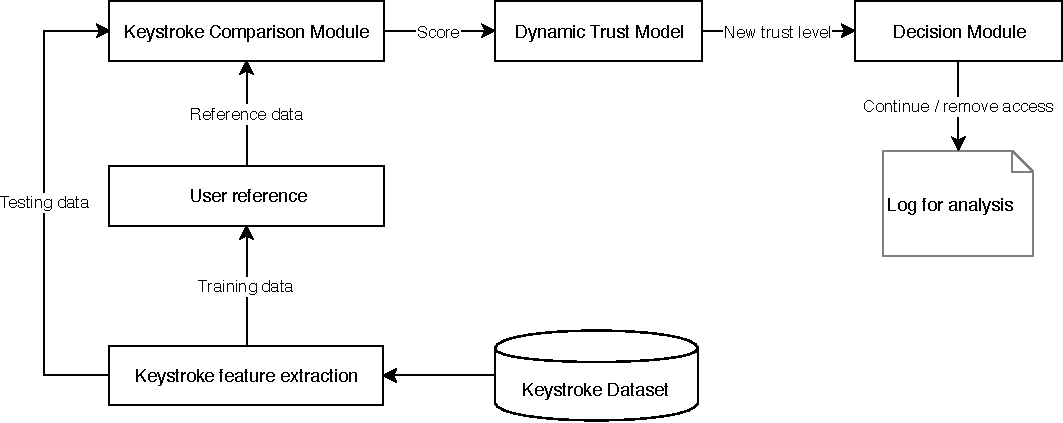
\includegraphics[width=0.9\textwidth]{figures/CA-diagram.pdf}
    \caption{Generalized diagram of the CA system's structure.}
    \label{fig:CA-diagram}
\end{figure}


\subsection{Feature extraction and references}
\label{sec:system-design-CA-ref}
Six features are utilized in the CA system, namely keycodes, monograph durations as well as PP, PR, RP and RR latencies from digraphs.
While certain systems in literature exclude monographs in their analysis, we found it necessary to consider them in our system.
If monographs were ignored, an attacker could wait for 1500 ms between keystrokes in order to avoid typing digraphs.
This would result in the system having little to no features available for comparison, even if the user typed a full block of monographs.
Including monographs features helps mitigate this security issue.

\begin{table}[h]
\centering
\begin{tabular}{|l|l|}
\hline
Monograph & Digraph\\ \hline
- Keycode & - Keycode\\
- Hit count & - Hit count\\
- $\text{Duration}_{\text{Mean}, \sigma} $& - $\text{PP}_{\text{Mean}, \sigma}$\\
& - $\text{PR}_{\text{Mean}, \sigma}$  \\
& - $\text{RP}_{\text{Mean}, \sigma}$ \\
& - $\text{RR}_{\text{Mean}, \sigma}$
\\ \hline
\end{tabular}

\caption{The structure of the references used in our system, where $\sigma$ is the standard deviation of recorded durations/latencies.}
\label{tab:CA-reference-structure}
\end{table}
\Cref{tab:CA-reference-structure} shows how these features are used in the reference.
For every n-graph occurring during enrollment, the system only stores the \textit{mean} and \textit{standard deviation} of the feature's recorded timing values, as well as its keycode and hit count.
The hit count keeps track of how many times each mono- or digraph occurred in enrollment.
All features are extracted as described in \Cref{sec:system-design-dataset}.
%Keycodes can also be considered a feature, but since all comparisons rely on identical keycodes, we will consider the durations and latencies.


As human behavior is prone to inconsistencies, removing outlier values can give more accurate representations of how a user typically behaves.
In PA systems, it is possible to remove outlier timing values from probe blocks, as each n-graph can have multiple recorded occurrences.
This is generally not the case for CA systems, as the trust level must be adjusted after every recorded keystroke.
However, it is possible to remove outliers from the CA reference.
We chose to so since our classifier relies on standard deviation, which causes it to be negatively affected by outliers.
For every feature in the reference, we removed outliers using Interquartile Range.
This was done within the scope of one feature. 
In other words, if a key were pressed only once and its duration were an outlier compared to other keys in the reference, it would still not be removed.
However, if the key had several occurrences, and therefore several durations, outlier durations would be removed if present.


\subsection{Comparison}
\label{sec:system-design-CA-matching}
When processing a keystroke, its extracted features are handled by the Keystroke Comparison Module which compares them to the genuine user's reference using a distance measure.
The comparison is performed by computing the dissimilarity score $sc$ between the probe timing features $p$ and the mean duration $\mu$ of the corresponding features from the same keycode in the reference.
This is calculated using the following formula:
$$ sc=\frac{1}{n}\sum_{i=1}^{n}\frac{|p_i-\mu_i|}{\sigma_i} $$
where $i$ is a specific feature, $n$ is the amount of available \textit{timing features} and $\sigma$ is the \textit{standard deviation} of the reference features.
Our implementation makes a distinction between monographs and digraphs in the sense that they produce two separate scores.
In practice, this causes $n$ to either be 1 (monograph duration) or 4 (digraph latencies).
For digraphs, this means that the score is the mean of the distances computed for the PP, PR, RP and RR latencies.

The formula is a variant of the Scaled Manhattan Distance, as described by Killourhy and Maxion \cite{Killourhy}.
They compared the performance of 14 different classifiers on static text keystroke dynamics, where Scaled Manhattan Distance achieved the best Equal Error Rate.
%Their variant uses mean absolute deviation for scaling the scores, while we have chosen standard deviation, 
This distance metric shows the dissimilarity between the probe and reference, and is used directly as the score input to the trust model.


\subsection{Trust model and decision module}
The trust model used in our system is a variant of the one presented by Mondal \cite{mondal}.
We have made certain changes to make it fit our system, and eliminated one parameter which was not used in our analysis.
\Cref{alg:trust-model} shows our implementation of the trust model.
Perhaps the most notable change is the fact that the function is inverted horizontally, as seen in \Cref{fig:sigmoids}.
This was a necessary feature due to having a dissimilarity score as input.

\begin{algorithm}[htbp]
 \KwData{\\
 $sc_i\gets$ Dissimilarity score for $i^{th}$ action\\
 $A\gets$ Threshold for reward or penalty\\
 $B\gets$ Width of sigmoid function\\
 $C\gets$ Maximum reward and penalty\\
 $Trust_{i-1}\gets$ Trust level after $(i-1)^{th}$ action\\
 }
 \KwResult{\\$Trust_i\to$ Trust level after $i^{th}$ action}
 \Begin{
 \begin{equation}
 \Delta_T(sc_i) = \text{min}\{-C + (\frac{C*2}{1 + \text{exp}(\frac{sc_i-A}{B})}), C\}
 \label{eq:delta-trust}
 \end{equation}
 \begin{equation}
 Trust_i = \text{min}\{\text{max}\{Trust_{i-1} + \Delta_T(sc_i), 0\}, 100\}
 \end{equation}
 }
 \caption{Algorithm for the Trust Model}
\label{alg:trust-model}
\end{algorithm}

\begin{figure}[!htbp]
  \begin{subfigure}[b]{0.5\textwidth}
    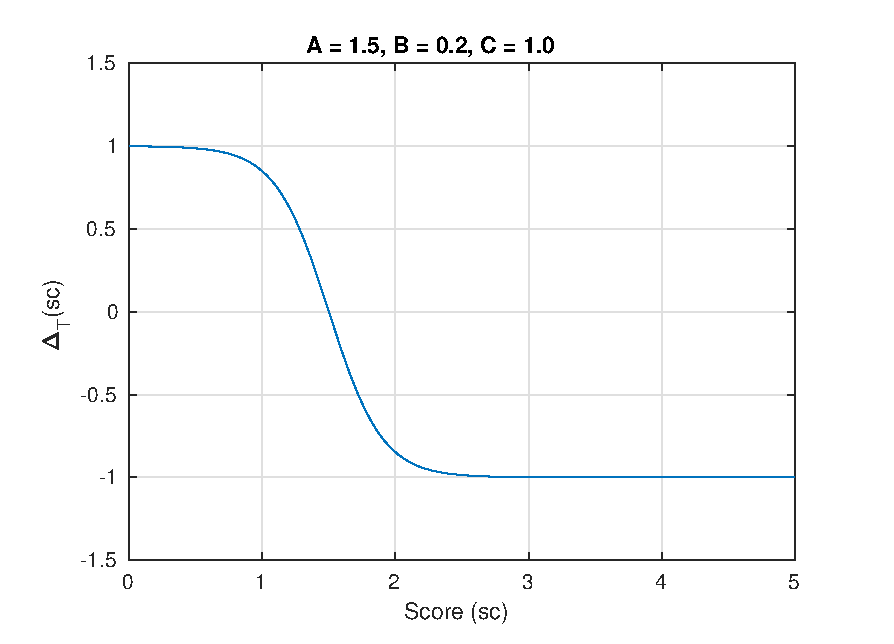
\includegraphics[width=\textwidth, height= 0.3\textheight]{figures/sigmoid1.eps}
    \label{fig:sigmoid1}
  \end{subfigure}
  \hfill
  \begin{subfigure}[b]{0.5\textwidth}
    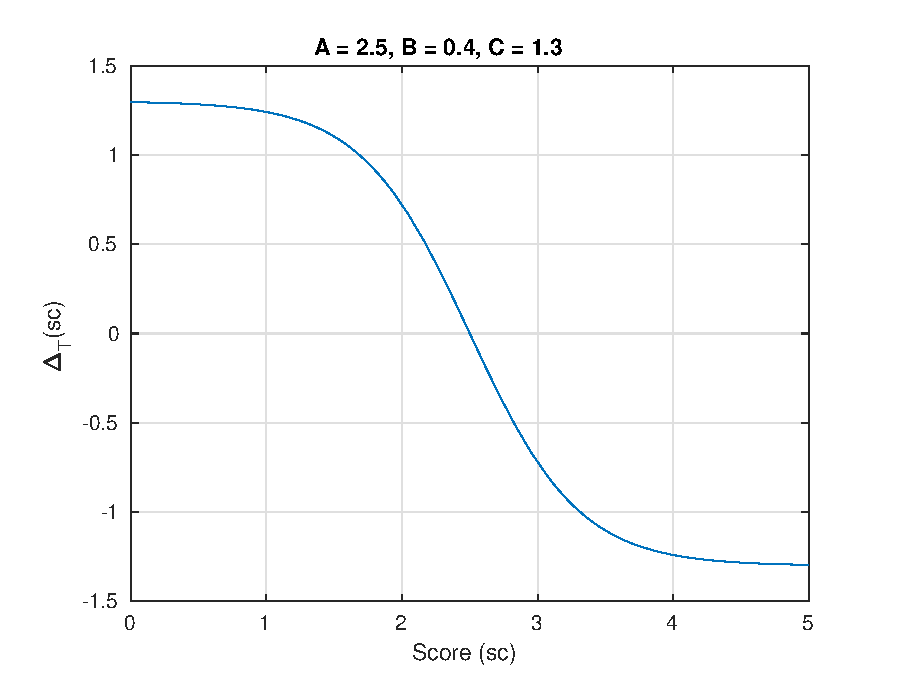
\includegraphics[width=\textwidth, height=0.3\textheight]{figures/sigmoid3.eps}
    \label{fig:sigmoid2}
  \end{subfigure}
  \caption{Examples of how the score would affect the trust level using different parameters for \Cref{eq:delta-trust}.}
  \label{fig:sigmoids}
\end{figure}

As mentioned in \Cref{sec:system-design-CA-matching}, monograph scores and digraph scores are separated.
In practice, this means that the $2^{\text{nd}}$ monograph of a valid digraph produces \textit{two} scores.
One score represents the monograph, while the other represents the digraph.
Therefore, a digraph produces \textit{three} scores in total: 2 monograph scores + 1 digraph score. 
This brought in the question of how to handle digraph actions at the lockout threshold.
For example, let the current trust level $Trust_{i-1} = 90.3$ and lockout threshold $T_{\text{lockout}} = 90$.
It is then possible that the next monograph score causes $Trust_i = 89.6$.
However, if the system locks the user out at that point, it disregards the fact that the monograph may be the $2^{\text{nd}}$ component of a digraph.
This issue is highlighted when the digraph score would have raised the trust level back to a value above $T_{\text{lockout}}$, for example $Trust_i = 90.2$.
Therefore, when observing digraph actions, the Decision Module locks the user out only if $Trust_i < T_{\text{lockout}}$ after considering both the monograph \textit{and} digraph scores of the keystroke.

\section{PA system}
The foundation of our PA system is based on that of Ferreira and Santos \cite{superResults}.
Some of their features, such as "progressive learning" has been excluded from our implementation.
When three consecutive probe blocks were accepted, their system would update the user's reference, infusing said probes into it in order to keep the reference up to date with the genuine user's most recent behavior.
The reason for not including this feature is threefold:
\begin{itemize}
    \item The dataset we used for analysis was collected over the course of about one week per user. The user's typical behavior is not expected to be significantly changed that quickly, eliminating the need for an adaptive reference.
    \item Even if this would slightly improve performance, our goal is not to necessarily create high performing CA or PA systems. 
    Instead, it is to observe the effect of combining them regardless of what their individual performances are.
    \item Updating the user's reference several times when testing system performance would severely impact processing time for full test runs. 
    This would in turn impact the amount of different parameter sets we would be able to test in the project's analysis phase.
    Therefore, we chose to prioritize testing as many sets of parameters as possible over including this feature.
    In a real-time system, the extra computational work would be trivial due to larger time periods between each update.
\end{itemize}

\begin{figure}[h]
    \centering
    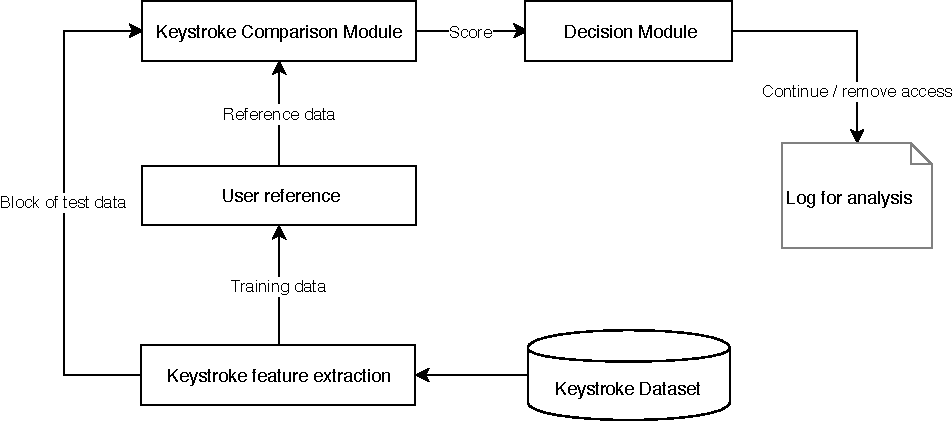
\includegraphics[width=0.9\textwidth]{figures/PA-diagram.pdf}
    \caption{Generalized diagram of the PA system's structure.}
    \label{fig:PA-diagram}
\end{figure}

The PA system is displayed in \Cref{fig:PA-diagram}.
Its structure is similar to that of the CA system, though the PA system has no Trust Module. 
Also, a block of keystroke features is fed as input to the Keystroke Comparison Module, as opposed to one keystroke at a time in the CA system.
The following subsections further describe the different components of the PA system.

\subsection{Feature extraction and references}
We have used the same reference for our PA system as described in \Cref{sec:system-design-CA-ref}, however, a different set of features is considered.
Ferreira and Santos \cite{superResults} consider monograph durations, digraph PP and RP latencies, as well as PP latencies for trigraphs and tetragraphs (4-graphs).
In order to soften computational impact, trigraphs and tetragraphs were excluded from our system.
This left us with the features listed in \Cref{tab:PA-reference-structure}.
Probes are formed using the same structure.

\begin{table}[h]
\centering
\begin{tabular}{|l|l|}
\hline
Monograph & Digraph\\ \hline
- Keycode & - Keycode\\
- Hit count & - Hit count\\
- $\text{Duration}_{\text{Mean}} $& - $\text{PP}_{\text{Mean}}$\\
& - $\text{RP}_{\text{Mean}}$ \\
\hline
\end{tabular}

\caption{The structure of the probes and references used in our PA system.}
\label{tab:PA-reference-structure}
\end{table}

\subsection{Comparison}
\todo{Explain the term "n-graph", possibly also mono and digraph.}
The Comparison Module uses the R and A measures presented by Gunetti and Picardi \cite{gnp}, which have been adopted by several other authors, including Ferreira and Santos \cite{superResults}.
These two measures are calculated for every sample, and are combined to produce a final distance.
Following is a description of how these distances are produced in our system.

\subsubsection{R-distance}

After the current user has typed an amount of keystrokes equal to the block length used by the system, the features in \Cref{tab:PA-reference-structure} are extracted from the block sample to form a probe.
The Keystroke Comparison Module then finds all n-graphs that are shared between the probe and the genuine user's reference.
The shared n-graphs are separated into one set for monographs and one set for digraphs which are processed individually.
\todo{Correct "R measure" to "R-distance" throughout.}
To calculate the R (relative) distance of a probe, the shared monographs and digraphs are extracted into probe and reference feature vectors sorted by durations and latencies, respectively.
For every feature vector (monograph durations, digraph PP and digraph RP), the position of each n-graph in the probe is compared to the same n-graph's position in the reference vector.
This results in a \textit{position distance} being produced for each n-graph.
The R measure is then calculated by summing the position distances of all n-graphs per feature vector, and normalizing the result.
The normalization allows us to compare and combine R measures calculated from feature vectors of different lengths. This is useful as there may be more digraphs shared than monographs, or vice versa.
The normalization is performed by dividing the summed position distances by the maximum possible disorder in an array of the same length as the respective feature vector.

\begin{table}[h]
\centering
    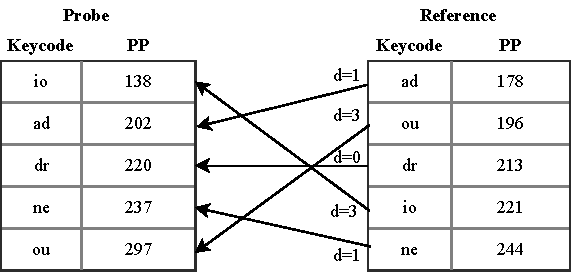
\includegraphics[width=0.6\textwidth]{figures/R-measure_OC.pdf}
    \caption{Calculation of the relative distance between the digraphs of the word "authentication" which are shared between the probe and reference.}
    \label{fig:R-measure}
\end{table}

An example of R-distance calculation for PP latencies is shown in \Cref{fig:R-measure}. The example is based on that of the R and A measures' original authors \cite{gnp}.
Five of the digraphs from the probe were found in the reference, and so the shared digraphs are sorted by their latencies.
The digraphs' summed position distances is $1 + 3 + 0 + 3 + 1 = 8$.
With there being five digraphs shared between the probe and reference, the maximum order of the feature vector is $(5^2 - 1)/2 = 12$.
Thus, the R-distance is $8/12 = 0.666$.
In our PA system, the same procedure would be performed for monograph durations and RP latencies as well.

When an R-distance is produced for each of our three probe feature vectors, the distances are combined.
This is done by means of weighed summation.
The more durations/latencies are available in a feature vector, the higher weight it is given.
This ensures that the feature which has more data to base its R-distance on, and thus is likely to be more accurate, is prioritized.

\Cref{eq:R-combination} shows the weighted summation where $R_n, R_m$ and $R_p$ are R-distances of durations, PP latencies and RP latencies, respectively.
Furthermore, $X = \text{max}(N, M, P)$ where $N$ is the number of recorded durations, while $M$ and $P$ are the respective number of recorded PP and RP latencies divided by 2.
This division is performed to avoid an unfair weighing of digraphs, as digraphs produce \textit{two} timing features.

\begin{equation}
\label{eq:R-combination}
    R_{\text{total}} = R_n \times \frac{N}{X} + R_m \times \frac{M}{X} + R_p \times \frac{P}{X}
\end{equation}

Where we have based our weighting on total number of durations/latencies per feature vector, the original authors use the \textit{number of shared n-graphs}.
The reason for changing this, is that our dataset contains a large variety of behaviors, as the data was collected in an unconstrained environment.
A consequence is that some participants were for example playing games during data collection.
When playing these games, very few unique keys were pressed, though they were pressed rapidly over long periods of time.
In the case where a block would consist mostly of only one character being pressed repetitively, which is a realistic situation with our dataset, only a few monographs other than the repeated key could heavily shift the weight in favor of monographs.
A weighing like this could be detrimental, as a great amount of valuable information from the recorded digraphs of the repeated key would have only a small impact on the result.

On the other hand, a consequence of our weighting scheme is that monographs will always be prioritized over digraphs.
With a block length of 100, the amount of available monographs would be 100, while there would be at most $100 - 1 = 99$ digraphs.
Prioritizing monograph durations is supported by Pinto et al. \cite{Pinto2014}, who found that using the following weights produced the overall best results: 42\% for monograph durations, 24\% for digraph RP, 16\% digraph PP, 10\% trigraph PP and 8\% tetragraph PP latencies.
However, their study was performed on a limited dataset of 10 participants where most of them were software developers.

\subsubsection{A-distance}
As the R-distance only accounts for \textit{relative} speeds as mentioned in \Cref{sec:related-statistical-approaches}, the A-distance considers the \textit{absolute} timing values, and measures the distances between these.
%When combining the R- and A-distances, we achieve a classifier which both takes into account that the genuine user may experience a condition causing them to generally type faster or slower than usual, in addition to detecting imposters who may type in a similar rhythm as the user, but at different speeds.
When combining the R- and A-distances, we achieve a classifier which both considers \textit{typing rhythm} using the R-distance, as well as raw typing speed.

When calculating the A-distance between a probe and a reference, we reuse the feature vectors from the R-distance calculation, however the fact that they are sorted by duration/latency is irrelevant.
To calculate the A-distance, the system first has to decide which n-graph durations/latencies from the probe are to be considered as \textit{similar} to those in the reference.
When comparing for instance monographs, the system would regard durations as \textit{similar} if the longer duration divided by the shorter duration is between 1 and an arbitrary threshold.
Using standard deviation instead of a fixed threshold would be a viable option, but the fixed threshold allows comparison between monographs with only one occurrence.

Gunetti and Picardi \cite{gnp} used 1.25 as the threshold for similarity, after testing different thresholds on a subset of their users.
While another threshold may be optimal for our dataset, we have also decided to use 1.25 for our system, as achieving optimal PA or CA performance is not the purpose of this project.

\begin{table}[h]
\centering
\begin{tabular}{rcccl}
 \bf Digraph & \bf Probe & \bf Ref. & \bf Calculation &  \\
 io & 138 & 221 & $221/138=1.60$ &  \\
 ad & 202 & 178 & $202/178=1.13$ & (similar) \\
 dr & 220 & 213 & $220/213=1.03$ & (similar) \\
 ne & 237 & 244 & $244/237=1.03$ & (similar) \\
 ou & 297 & 196 & $297/196=1.52$ & \\
\end{tabular}
\caption{Similarities between trigraphs from \cref{fig:R-measure}.}
\label{tab:A-distance-similar}
\end{table}

\todo{Use times symbol all over the document.}




\section{Combined system}



%\subsection{Outliers}
%----
%In PA systems, it is possible to remove outlier timing values from probes, as each n-graph can have multiple recorded durations or latencies.
%This is generally not the case for CA systems, as a the trust level is adjusted after every recorded keystroke.
%However, it is possible to remove outliers from the CA reference.
%When testing the CA system with the Scaled Manhattan Distance, its ANGA and ANIA values dropped significantly, down to 1116 and 173, respectively.
%While detecting imposters after only 173 keystrokes on average is a very good result seen in isolation, locking out the genuine users after 1116 keystrokes on average is far too often to be seen as a practically viable system.
%We were able to adjust parameters so that the ANGA was raised to approximately 4157, though the ANIA was also raised to 638.
%We were unable to separate or raise the values much further beyond this point.
%
%A plausible explanation for this is that Scaled Manhattan Distance already takes outliers into account by using standard deviations.
%When outliers were removed from the reference, the standard deviations for several n-graphs were drastically lowered, causing the classifier to be too strict. 
%In essence, it was demanding much less deviation from the mean than what can be realistically expected from the genuine user's natural behavior.
%Therefore, we decided to keep outliers in the reference for this version of the system.




%Our goal was to investigate the impact of combining periodic and continuous authentication.
%
%
%
%As our goal is not to achieve the best performing system, but rather to s